% To be compiled with pdf LaTeX
% This file is to be included into master file via \input command
% Note that there is no \begin{document} \end{document} brackets!

\newpage
\section{Control}
\label{sec:control}

%\subsection{Nomenclature}

%\mbox{}

%$\bm{s}$ - vector of wavefront sensor measurements concatenated both for x- and
%y-slopes and from different sensors, [pixels or radians of slope].
%\\

%$\phi(\bm{x})$ - continuous wavefront phase distribution in exit pupil, [rad].
%\\

%$\{ \phi(\bm{x})_{i} \}_{i=1}^{\infty}$ - set of basis functions for the exit
%pupil phase expansion, [rad].
%\\

%$\bm{x}_{Sc}$ - vector of discretized phase values in the telescope exit pupil
%for the light coming from a science object, [rad].
%\\

%$\hat{\bm{x}}_{0}$ - estimate of vector of discretized phase values in the
%telescope exit pupil
%for the light coming from a science object, [rad].
%\\

%$\bm{x}$ - vector of discretized phase values in the telescope exit pupil for
%the light from a guide star to wavefront sensor, concatenated for all sensors,
%[rad].
%\\

%$\bm{n}_{s}$ - vector of sensor readout noise concatenated from all sensors,
%[pixels or radians of slope].
%\\

%$\{ f(\bm{x})_{i} \}_{i=1}^{\#actuators}$ - set of continuous phase influence
%functions of a deformable mirror, [rad].

%$\bm{c}$ - vector of control commands concatenated from all correctors (DMs,
%tip-tilt mirrors, moving stages), [control units, e.g. V].
%\\

%$\hat{\bm{c}}$ - vector of control commands estimated from a control algorithm.
%\\

%$\bm{n}_{a}$ - vector of actuator noise concatenated from all correctors,
%[control units].
%\\

%$\mathcal{E}$ - estimation (control) matrix.
%\\

%$\mathcal{G}$ - wavefront-to-WFS interaction matrix, [rad/slope].
%\\

%$\delta \mathcal{G}$ - error in the wavefront-to-WFS interaction matrix,
%[rad/slope].
%\\

%$\mathcal{D}$ - command-to-WFS interaction (``poke'') matrix, [control
%units/slope].
%\\

%$\delta \mathcal{D}$ - error in the command-to-WFS interaction matrix,
%[rad/slope].
%\\

%$\mathcal{F}$ - command-to-phase interaction (``influence function'') matrix,
%[control units/rad].
%\\

%$\delta \mathcal{F}$ - error in command-to-phase interaction (``influence
%function'') matrix, [control units/rad].
%\\

%$\langle \bm{x} \bm{x}^{T} \rangle$ - auto-covariance matrix of the guide star
%phase in exit pupil, [rad$^{2}$].
%\\

%$\langle \bm{x}_{Sc} \bm{x}^{T} \rangle$ - cross-covariance matrix of the
%science object and guide star phase in exit pupil, [rad$^{2}$].
%\\

%$\langle \bm{n}_{s} \bm{n}_{s}^{T} \rangle$ - auto-covariance matrix of the
%sensor readout noise, [slope$^{2}$].
%\\

%$\langle \bm{n}_{a} \bm{n}_{a}^{T} \rangle$ - auto-covariance matrix of the
%actuator noise, [control units$^{2}$].
%\\

\subsection{Linear system model and discretization}
\label{subsec:system-models}

In our treatment of an AO system modeling we follow closely the ``natural
modeling'' approach described in Refs.
\cite{WibergMaxGavel1,WibergMaxGavel2}. To begin with, we consider the simplest
case of a single-conjugate AO system, which is modeled through the following
fundamental inputs.
\begin{enumerate}
	\item A light source to be imaged with an AO system (the \emph{target})
	creates a continuous phase distribution $\phi_{0}(\bm{x})$ in the
  telescope entrance pupil,
	which is the accumulated phase distortion along the
  path from a light source to the telescope that includes atmospheric
  turbulence distortion. It is supposed that the
  autocorrelation function $\langle \phi_{0}(\bm{x}_{1}) \phi_{0}(\bm{x}_{2})
  \rangle_{\phi}$ is known.
  \item A set $\{ f_{i}(\bm{x}) \}_{i=1}^{\#ACT}$ ($\#ACT$ is the number of DM
  actuators) of the DM actuator influence
  functions projected as phase correction in the telescope entrance pupil. We
  will write these functions in vectorial form $\bm{f}(\bm{x})$. Note that, same
  as $\phi(\bm{x})$, these functions depend on the light source. The DM
  correction is assumed to be a linear combination of the influence functions:
  \begin{equation} \label{eq:dm-phase-correction}
		\phi_{DM}(\bm{x}) = \sum_{i=1}^{\#ACT} c_{i} f_{i}(\bm{x})
	\end{equation}
	or
	$$
	  \phi_{DM}(\bm{x}) = \bm{f}^{T}(\bm{x}) \bm{c},
	$$
	where $\bm{c}$ is the vector of DM correction commands.
  \item A wavefront sensor (WFS) accepts light from a \emph{reference} source
  not in general coinciding with the target. WFS is modeled as a linear
  mapping of the reference wavefront $\phi{x,y}$ in the entrance pupil to a
  set of sensor measurements:
  \begin{equation} \label{eq:wfs-measurement-operator}
    \bm{s} = \mathcal{M} [ \phi(\bm{x}) ],
  \end{equation}
  where $\mathcal{M}$ is a linear \emph{measurement operator}.
  \index{measurement operator} The \emph{measurement equation}
  \index{measurement equation} describing the full linear sensor model is
  \begin{equation} \label{eq:measurement-equation}
	  \bm{s} = \mathcal{M} [ \phi(\bm{x}) + \delta \phi(\bm{x}) ] + \bm{n},
  \end{equation}
  where $\bm{n}$ is random sensor readout noise with known autocorrelation
  matrix $\langle \bm{n} \bm{n}^{T} \rangle_{n}$,
  $\delta \phi(\bm{x})$ is an additive aberration due to propagation from
  telescope entrance pupil to the exit pupil conjugate to the WFS location. We
  will assume for the moment that this aberration can be perfectly calibrated
  out, so $\delta \phi (\bm{x}) = 0$.
\end{enumerate}
This small set of parameters are enough to fully describe a linear model of an
AO system.

\subsection{Minimum Mean Square Error AO control}
\label{subsec:MMSE-control}

The goal of the \emph{Minimum Mean Square Error} (MMSE) \index{Minimum Mean
Square Error} AO control is to find a command vector $\hat{\bm{c}}$ such that
the DM correction minimizes the target wavefront mean square phase error
(\emph{quadratic cost}) \index{quadratic cost} in the
telescope entrance pupil
\begin{equation} \label{eq:mmse-cost}
	\langle J \rangle_{\phi,n} =
	\langle ||\phi_{0}-\phi_{DM}||^{2} \rangle_{\phi,n},
\end{equation}
where Hilbert space norm
\begin{equation} \label{eq:Hilbert-norm}
	|| a(\bm{x}) ||^{2} = [a(\bm{x}),a(\bm{x})] =
	\frac{1}{|A|} \int_{A} ds \, a^{2}(\bm{x}),
\end{equation}
is derived from the Hilbert space metric
\begin{equation} \label{eq:Hilbert-metric}
	[a(\bm{x}),b(\bm{x})] = \frac{1}{|A|} \int_{A} ds \, a(\bm{x}) b(\bm{x}),
\end{equation}
$A$ is the telescope entrance pupil domain (the \emph{aperture}),
\index{aperture} $|A|$ is the aperture area, and $\langle \rangle_{\phi}$
denotes averaging over joint statistics of the input turbulent wavefront and
the sensor noise. We can consider two cases of the quadratic cost
minimization: 1) \emph{DM fitting} \index{DM fitting} and 2) \emph{phase
estimation}. \index{phase estimation}

\subsubsection{DM fitting}

The DM fitting problem statement is:
given target wavefront phase $\phi_{0}(\bm{x})$ at the entrance pupil find the
DM command vector $\hat{\bm{c}}$ such that the deterministic wavefront error
is minimized:
\begin{equation} \label{eq:DM-fit-minimization}
	\hat{\bm{c}} = \arg \min_{\forall \bm{c}}
	||\phi_{0} - \bm{f}^{T} \bm{c}||^{2}.
\end{equation}
It is known from the theory of Hilbert spaces that the above equation is
equivalent to
\begin{equation} \label{eq:deterministic-orthogonality-principle}
	[\phi_{0} - \bm{f}^{T} \hat{\bm{c}}, \bm{f}] = 0,
\end{equation}
which is a form of the \emph{orthogonality principle} stating that
\begin{flushleft}
	\texttt{the optimal fitting error is orthogonal to the subspace spanned by
	the influence functions.}
\end{flushleft}
Solving Eq. (\ref{eq:DM-fit-minimization}) or the equivalent Eq.
(\ref{eq:deterministic-orthogonality-principle}) yields for the optimal
control command
\begin{equation} \label{eq:fitting-commands}
	\hat{\bm{c}} = [\bm{f},\bm{f}^{T}]^{\dagger} [\bm{f},\phi_{0}],
\end{equation}
where $[\bm{f},\bm{f}^{T}]$ is called \emph{Gramm matrix} of the function set
$\bm{f}(\bm{x})$, $^{\dagger}$ stands for pseudo inverse. The Gramm matrix is
square and is invertible in case the influence functions $\bm{f} (\bm{x})$ are
linearly independent. Since linear independence is not guaranteed for the real
DM influence functions, the filtered pseudo-inverse is used. Note that in case
of pseudo-inverse the orthogonality principle does not hold exactly. This,
however, is easily fixed if we redefine the influence functions as, e.g., a
subset of orthogonal singular modes of the Gramm matrix with sufficiently large
singular values.

The optimal \emph{fitting error} is \index{fitting error}
\begin{equation} \label{eq:fitting-error}
	J_{c} = [\phi_{0} - \bm{f}^{T} \hat{\bm{c}},\phi_{0} -
	         \bm{f}^{T} \hat{\bm{c}}]
\end{equation}
$$
  = [\phi_{0} - \bm{f}^{T} \hat{\bm{c}},\phi_{0}]
$$
$$
  = [\phi_{0},\phi_{0}] -
    [\bm{f}^{T},\phi_{0}] [\bm{f},\bm{f}^{T}]^{\dagger} [\bm{f},\phi_{0}],
$$
where we used Eqs. (\ref{eq:deterministic-orthogonality-principle}) and
(\ref{eq:fitting-commands}). The orthogonality principle states that the phase
can be presented as a sum of two mutually orthogonal \emph{controllable}
$\hat{\phi}_{0}$ and
\emph{uncontrollable} $\check{\phi}_{0}$ parts \index{controllable part}
\index{uncontrollable part}
\begin{equation} \label{eq:controllable-uncontrollable}
	\phi (\bm{x}) = \hat{\phi}_{0} (\bm{x}) + \check{\phi}_{0} (\bm{x}),
\end{equation}
where
\begin{equation} \label{eq:controllable-projection}
	\hat{\phi}_{0} = \bm{f}^{T} [\bm{f},\bm{f}^{T}]^{\dagger} [\bm{f},\phi_{0}] =
	\mathcal{F} \phi_{0},
\end{equation}
\begin{equation} \label{eq:uncontrollable-projection}
	\check{\phi}_{0} = \phi_{0} - \mathcal{F} (\phi_{0}) =
	(\mathcal{I - F})\phi_{0}
\end{equation}
and $\mathcal{F},\mathcal{I - F}$ are orthogonal projection operators on,
respectively, \emph{controllable} and \emph{uncontrollable subspaces} of the
influence function set $\bm{f}$. \index{controllable subspace}
\index{uncontrollable subspace} Note that the dimension of the controllable
subspace is finite, so either $\hat{\bm{c}}$ or $\bm{\phi}_{0} =
[\bm{f},\phi_{0}]$
are the natural discrete representations for the controllable part of the
wavefront phase, the only part of interest in the AO control.

\subsubsection{Phase estimation}

The phase estimation problem statement is: given sensor measurements $\bm{s}$
find an estimate $\tilde{\phi}_{0}(\bm{x})$ of the target source phase in the
entrance pupil such
that the mean square error is minimized over the measurement statistics, in
our case, the joint turbulence and sensor noise statistics:
\begin{equation} \label{eq:estimation-minimization}
	\tilde{\phi}_{0} =
	\arg \min_{\forall \mathcal{E}}
	\langle
	||\phi_{0} - \mathcal{E} \bm{s}||^{2}
	\rangle_{\phi,n},
\end{equation}
where $\mathcal{E}$ is the linear estimator operator.
Analogously to the deterministic orthogonality principle the \emph{orthogonality
principle of statistical estimation} \index{orthogonality principle} states that
\begin{flushleft}
	\texttt{optimal estimator error is statistically orthogonal to the
	measurements,}
\end{flushleft}
i.e., for our case
\begin{equation} \label{eq:statistical-orthogonality-principle}
	\langle ( \mathcal{E}\bm{s} - \phi_{0} ) \bm{s}^{T} \rangle_{\phi,n} = 0.
\end{equation}
Solving Eq. (\ref{eq:estimation-minimization}) or its equivalent
(\ref{eq:statistical-orthogonality-principle}) yields
\begin{equation} \label{eq:phase-estimate}
	\tilde{\phi}_{0} = \langle \phi_{0} \bm{s}^{T} \rangle_{\phi,n}
	                   \langle \bm{s} \bm{s}^{T} \rangle_{\phi,n}^{-1} \bm{s}.
\end{equation}
The optimal estimation error is
\begin{equation} \label{eq:estimation-error}
  \langle J_{e} \rangle_{\phi,n} =
	\langle
	[\phi_{0} - \tilde{\phi}_{0},\phi_{0} - \tilde{\phi}_{0}]
	\rangle_{\phi,n}
\end{equation}
$$
  = \langle [\phi_{0} - \tilde{\phi}_{0},\phi] \rangle_{\phi,n}
$$
$$
  = \langle [\phi_{0},\phi_{0}] \rangle_{\phi,n} -
    \langle \phi_{0} \bm{s}^{T} \rangle_{\phi,n}
	  \langle \bm{ss}^{T} \rangle_{\phi,n}^{-1}
	  \langle \bm{s} \phi_{0} \rangle_{\phi,n},
$$
where Eqs. (\ref{eq:statistical-orthogonality-principle}),
           (\ref{eq:phase-estimate}) were used.

Comparison Eq. (\ref{eq:phase-estimate}) with Eq.
(\ref{eq:controllable-projection}) reveals the fact that
the statistical estimation and fitting problems have essentially the same
structure. Indeed, Eq. (\ref{eq:phase-estimate}) coincides with Eq.
(\ref{eq:controllable-projection}) for the controllable part of the wavefront
after substitutions
$$
  \langle \bm{s} \phi_{0}(\bm{x}) \rangle_{\phi,n} \rightarrow
  \bm{f}(\bm{x}), \,\,
  \texttt{(estimation influence functions)},
$$
$$
  \langle \bm{s} \bm{s}^{T} \rangle_{\phi,n} \rightarrow [\bm{f},\bm{f}^{T}],
  \,\, \texttt{(estimation Gramm matrix)},
$$
$$
  \bm{s} \rightarrow [\bm{f},\phi_{0}], \,\,
  \texttt{(projection on measurements)},
$$
$$
  \tilde{\phi}_{0} \rightarrow \hat{\phi}_{0}, \,\,
  \texttt{(observable part of wavefront)}.
$$
Thus, there exists another, ``observable-unobservable'', orthogonal
decomposition of the input wavefront (see Ref. \cite{WibergMaxGavel2} for the
proof):
\begin{equation} \label{eq:observable-unobservable}
	\phi_{0} (\bm{x}) = \tilde{\phi}_{0} (\bm{x}) + \bar{\phi}_{0} (\bm{x}),
\end{equation}
where
\begin{equation} \label{eq:observable-projection}
	\tilde{\phi}_{0} = \langle \bm{s}^{T} \phi_{0} \rangle_{\phi,n}
	             \langle \bm{s} \bm{s}^{T} \rangle_{\phi,n}^{-1}
	             \mathcal{M} \phi = \mathcal{O} \phi,
\end{equation}
\begin{equation} \label{eq:unobservable-projection}
	\bar{\phi}_{0} = \phi_{0} - \mathcal{O} \phi.
\end{equation}
Again, the observable part of the wavefront, the only part of interest for AO
wavefront sensing, is finite-dimensional, and either $\bm{s}$ or
$\bm{w} = \langle \bm{s} \bm{s}^{T} \rangle_{\phi,n}^{-1} \bm{s}$ can be
naturally used as discrete representations of the $\tilde{\phi}_{0}$.

\subsubsection{Joint estimation and fitting, separation principle}

Now consider the problem of joint estimation and fitting, namely, given
measurement $\bm{s}$ and a set of influence functions $\bm{f}(\bm{x})$ find the
control commands $\hat{\bm{c}}$ such that
\begin{equation} \label{eq:joint-minimization}
	\hat{\bm{c}} = \mathcal{C} \bm{s} =
	\arg \min_{\forall \mathcal{C}}
	\langle
	|| \phi_{0} - \bm{f}^{T} \mathcal{C} \bm{s} ||^{2}
	\rangle_{\phi,n},
\end{equation}
where $\mathcal{C}$ is the estimator matrix creating linear mapping from the
set of sensor measurements to the set of DM commands. Expanding the norm in Eq.
(\ref{eq:joint-minimization}) one gets
\begin{equation} \label{eq:cost-expansion}
  || \phi_{0} - \hat{\phi} ||^{2} =
  || (\phi_{0} - \tilde{\phi}_{0}) + (\tilde{\phi}_{0} - \hat{\phi}) ||^{2}
\end{equation}
$$
 = || \bar{\phi}_{0} ||^{2} +
   2 [\bar{\phi}_{0},
     \tilde{\phi}_{0} - \bm{f}^{T} \mathcal{C} \bm{s} ] +
   || \tilde{\phi}_{0} - \bm{f}^{T} \mathcal{C} \bm{s} ||^{2},
$$
$$
  \hat{\phi} = \bm{f}^{T} \mathcal{C} \bm{s}.
$$
$
\langle
[\bar{\phi}_{0}, \tilde{\phi}_{0} - \bm{f}^{T} \mathcal{C} \bm{s} ]
\rangle_{\phi,n} = 0
$
for an optimal phase estimate $\tilde{\phi}_{0}$ because of the orthogonality
principle (\ref{eq:statistical-orthogonality-principle}). Thus
\begin{equation} \label{eq:separated-cost}
	\langle J \rangle_{\phi,n} =
	\langle || \phi - \hat{\phi} ||^{2} \rangle_{\phi,n}
\end{equation}
$$
  = \langle || \bar{\phi}_{0} ||^{2} \rangle_{\phi,n} +
    \langle
    || \tilde{\phi}_{0} - \bm{f}^{T} \mathcal{C} \bm{s} ||^{2}
    \rangle_{\phi,n},
$$
which is known as the \emph{separation principle of the quadratic control}.
\index{separation principle}
Eq. (\ref{eq:separated-cost}) shows that the overall error can be minimized
in two independent steps:
\begin{enumerate}
	\item Find the observable part of the target phase $\tilde{\phi}_{0}$ from
	Eq. (\ref{eq:phase-estimate}).
  \item Since $\tilde{\phi}_{0}$ is not a stochastic quantity, the $\langle
  \rangle_{\phi,n}$ brackets can be dropped for the second term reducing its
  minimization to deterministic fitting of the actuator influence
  functions to the phase estimate according to Eq. (\ref{eq:fitting-commands}).
\end{enumerate}
Following this path, i.e. substituting Eq. (\ref{eq:phase-estimate}) into Eq.
(\ref{eq:fitting-commands}), we get for the optimal reconstructor matrix
\begin{equation} \label{eq:optimal-reconstructor}
	\hat{\mathcal{C}} = [\bm{f},\bm{f}^{T}]^{\dagger}
	                    [\bm{f}, \langle \phi_{0} \bm{s}^{T} \rangle_{\phi,n} ]
	                    \langle \bm{s} \bm{s}^{T} \rangle_{\phi,n}^{-1}.
\end{equation}
The error for this reconstructor is
\begin{equation} \label{eq:reconstruction-error}
	\langle \hat{J} \rangle_{\phi,n} =
	\langle \bar{\phi}_{0} \rangle_{\phi,n} +
	\langle \check{\tilde{\phi}}_{0} \rangle_{\phi,n},
\end{equation}
where the first term is the phase estimation error given by Eq.
(\ref{eq:estimation-error}), second term is the fitting error of the
observable phase to the influence functions and is given by Eq.
(\ref{eq:fitting-error}) after substituting $\tilde{\phi}_{0}$ instead of
$\phi_{0}$.

Another important result derived in Ref. \cite{WibergMaxGavel2} concerns with
the estimate of the reconstruction error due to non-optimal reconstruction
matrix:
\begin{equation} \label{eq:non-optimal-reconstruction-error}
	\langle J \rangle_{\phi,n} - \langle \hat{J} \rangle_{\phi,n} =
	\texttt{Tr} \left\{
	[\bm{f},\bm{f}^{T}]
	( \mathcal{C} - \hat{\mathcal{C}} )
	\langle \bm{s} \bm{s}^{T} \rangle_{\phi,n}
	( \mathcal{C} - \hat{\mathcal{C}} )^{T} \right\},
\end{equation}
where $\mathcal{C}$ is the arbitrary control matrix that is not computed
according to prescription (\ref{eq:optimal-reconstructor}) and
$\langle J \rangle_{\phi,n}$ is the corresponding reconstruction error.

\subsubsection{Estimator for projected wavefront}

A modification of the phase estimation algorithm is needed for the situation
when it is necessary to find an estimate of the input phase part extractable
from $\phi(\bm{x})$ by a projection operation
\begin{equation} \label{eq:projection}
	\phi_{p}(\bm{x}) = \mathcal{P} ( \phi_{0} (\bm{x}) ),
\end{equation}
where $\mathcal{P}$ is a linear \emph{projection operator}. \index{projection
operator} Examples of such an operator are the controllable/uncontrollable
$\mathcal{F,(I-F)}$
projectors discussed above, the high-pass and low-pass spatial filters that
are an indispensable part of the GMT LTAO control strategy to be discussed
later in this document.

The optimal minimum least squares estimator for
$\mathcal{P} (\phi_{0})$  wavefront
instead of $\phi_{0}$ is derived from the minimization problem
\begin{equation} \label{eq:projected-estimation}
	\mathcal{E}_{p} = \arg \min_{\forall \mathcal{E}}
	                  \langle |\mathcal{P} (\phi_{0}) -
	                           \mathcal{E} \bm{s}|^{2} \rangle
\end{equation}
or from the orthogonality principle
\begin{equation} \label{eq:projected-estimator-orthogonality-principle}
	\langle (\mathcal{P} (\phi_{0}) -
	         \mathcal{E}_{p} \bm{s}) \bm{s}^{T} \rangle = 0,
\end{equation}
which, due to linearity of $\mathcal{P}$, trivially yealds
\begin{equation} \label{eq:projected-estimator}
	\mathcal{E}_{p} = \mathcal{P(E)},
\end{equation}
where $\mathcal{E}$ is given by Eq. (\ref{eq:phase-estimate}). Interesting,
if Eq. (\ref{eq:projected-estimator}) is used to find an optimal estimate
of the controllable part $\hat{\phi}_{0}$ of the input phase, Eq.
(\ref{eq:optimal-reconstructor}) for the optimal joint reconstructor results.

\subsubsection{Information deficiency in the WFS model. Aliasing error.}

\mbox{}

Practical MMSE controllers prove to be sub-optimal due to
information deficiency in the underlying system models. The MMSE approach
is model-based, i.e. it relies on the internal mathematical representation of
the real system. It is the ultimate goal of the system modeling for the
MMSE-based AO control to build the internal model only on physically measurable
(calibratable) data. There are, however, multiple causes for the necessary
data to be un-measurable. A fundamental model deficiency is that only
finite-dimensional approximation of the sensor measurement operator
$\mathcal{M}$ is possible based on the measurable data because this operator
maps the infinite-dimensional space $\mathbb{H}$ of the wavefront phases
$\phi(\bm{x})$ onto finite-dimensional space $\mathbb{S}$ of the sensor
readouts. Assume there are orthogonal bases in both $\mathbb{H}$ and
$\mathbb{S}$. Since the dimensionality of the $\mathbb{H}$-basis is higher
than that of $\mathbb{S}$ there is no way to find such a pair of bases that
each $\mathbb{S}$ basis function maps onto exactly one $\mathbb{H}$ basis
function, i.e. generally all components of $\phi(\bm{x})$, low and high order,
act on (``alias with'') each WFS measurement $s_{i}$. The aliasing is not a
problem as long as the $\mathcal{M}$ operator is known exactly because in this
case the $\langle \phi_{0} \bm{s}^{T} \rangle$ and $\langle \bm{s} \bm{s}^{T}
\rangle$ catch the correct ``aliasing pattern''. One can, however, practically
measure only $\mathcal{M}(\mathcal{P}\phi)$, where $\mathcal{P}$ is the
projector on a finite-dimensional subspace of $\mathbb{H}$. The resulting
finite-dimensional measurement operator $\mathcal{MP}$, if substituted into
Eq. (\ref{eq:measurement-equation}) and then into Eq.
(\ref{eq:optimal-reconstructor}) will result in not quite correct aliasing
pattern prediction and thus in a suboptimal reconstructor. The corresponding
additional
\emph{aliasing error} \index{aliasing error} can be estimated through
Eq. (\ref{eq:non-optimal-reconstruction-error}) once exact or at least more
elaborated model for the true measurement operator $\mathcal{M}$ is known.

A natural choice for the finite dimensional measurement operator approximation
$\mathcal{MP}$ is when $\mathcal{P} = \mathcal{F}$, the projection on the
controllable subspace (see Eq. (\ref{eq:controllable-projection})). In this
case $\mathcal{MP} = \mathcal{M}\bm{f}^{T} = \mathcal{D}$, where $\mathcal{D}$
is the DM \emph{poke matrix} \index{poke matrix} that is measurable by
recording sensor readouts
due to action of a DM actuator controlled (``poked'') one at a time. Since,
generally, the controllable part of the wavefront reliably represents low
spacial frequency content of the wavefront aberrations, it is wise to apply
low-pass spatial filter to the reference wavefront $\phi$ falling on the
sensor in order to reduce the discrepancy between the true action
$\mathcal{M} (\mathcal{P}_{LP} \phi)$ of the low-pass filtered wavefront and
its prediction $\mathcal{MP} (\mathcal{P}_{LP} \phi)$ and thus the aliasing
error \cite{Poyneer1}. Note that the optimal reconstructor equation
(\ref{eq:optimal-reconstructor}) has to be modified by replacing $\bm{s} =
\mathcal{M} \phi$ with $\bm{s}_{LP} = \mathcal{M} ( \mathcal{P}_{LP} \phi )$,
which, in general, will increase the optimal reconstruction error. This
increase is, however, expected to be compensated with the much more
significant decrease of the aliasing error contribution.

\subsubsection{Dynamic and closed-loop control}

The MMSE controller described above is an oversimplified version of a real AO
control algorithm based on two fundamental simplifying assumptions:
\begin{itemize}
	\item \emph{Open-loop operation}: \index{open-loop operation} it is assumed
	that the sensor measures input signal in the exit pupil directly,
	without any correction elements in the optical path in front of the sensor.
	A real AO system rarely works in open-loop regime because of small dynamic
	range of the existing WFSs. The more practical \emph{closed-loop} operation
	assumes that all the correction elements (DMs, tip/tilt mirrors, etc.) are
	located in front of sensors and the latter measure the difference between
	the input signal (turbulent wavefront) and its correction by DMs. In this
	case the input to the WFS is not
	$\phi(\bm{x})$ but $\delta \phi(\bm{x})$ and the input to
	controller is not $\bm{s}$ but $\delta \bm{s}$, the \emph{error signal}.
	\index{error signal}
  \item \emph{Non-dynamic} operation: \index{non-dynamic operation} it is
  assumed that signals propagate through the control system instantaneously
  and without temporal shape distortions. In reality, dynamic effects exist in
  the system. Two most important of them are: 1) signal delays due to
  data transfers, CCD exposure/readout time and controller computation time,
  2) signal distortions due to finite temporal bandwidth of the correction
  mechanism actuators. The dynamic effects increase the residual error and may
  also lead to system instability in closed-loop regime. To introduce dynamic
  effects one has to consider all quantities to be time-dependent by adding
  $n$ sub-index, $n=1,...,\infty$, for discrete time.
\end{itemize}

\begin{figure}[htp]
\begin{center}
\begin{tabular}{c}
 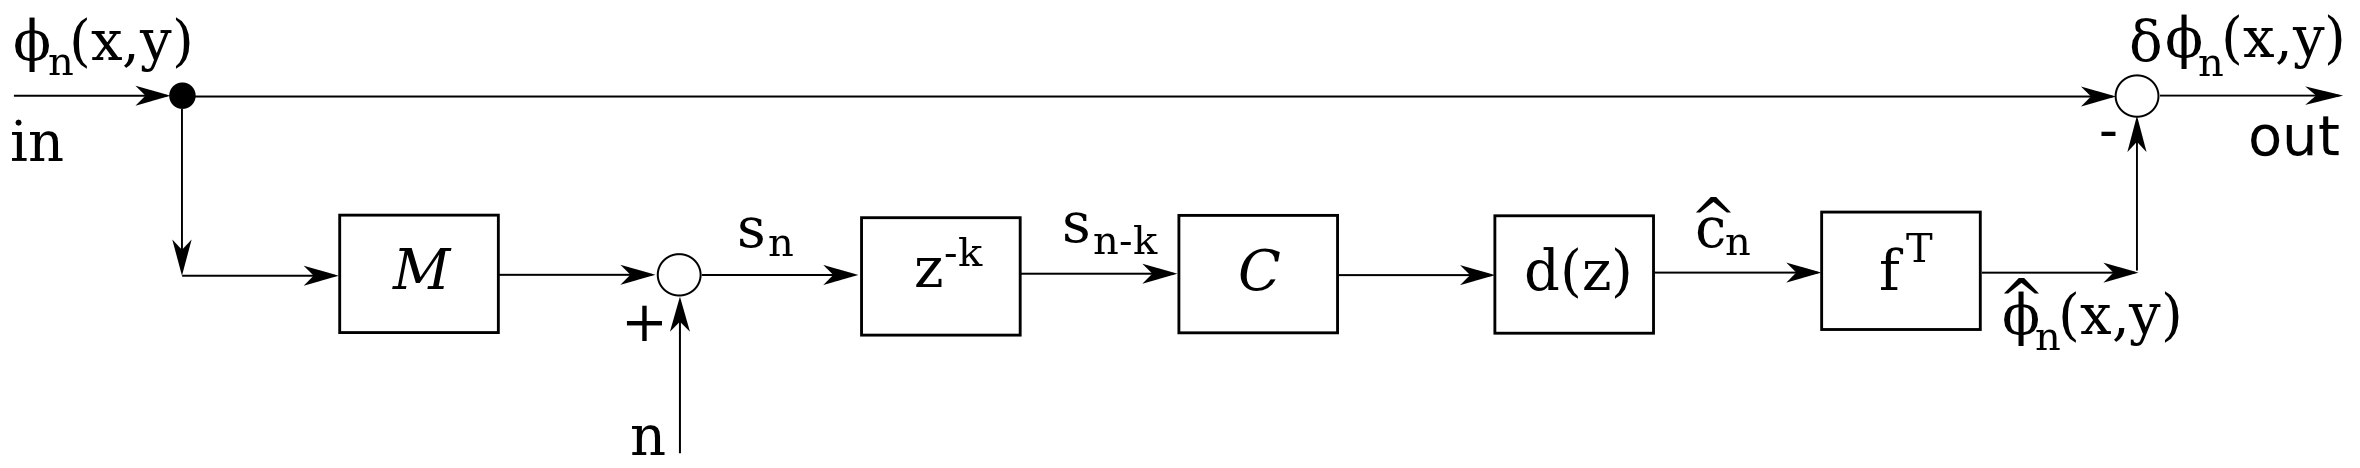
\includegraphics[width = 0.9\textwidth]{Forward.png} \\
 (a) \\
 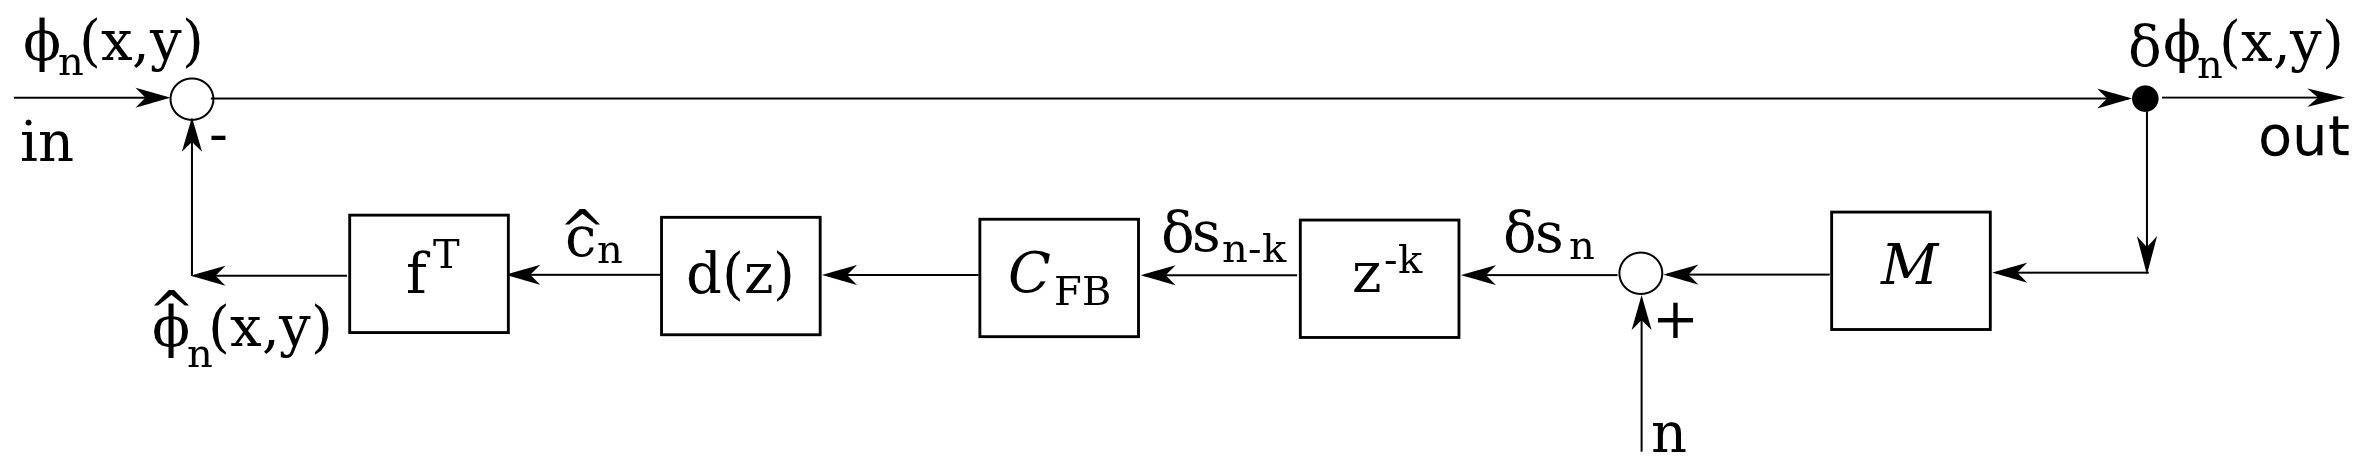
\includegraphics[width = 0.9\textwidth]{Back.png} \\
 (b) \\
\end{tabular}
\end{center}
\caption{Open-loop (a) and closed-loop (b) AO controller block diagrams.}
\label{fig:forward-back}
\end{figure}

Simplified signal block diagrams for an AO system in open-loop and closed-loop
configurations are shown on Fig. \ref{fig:forward-back}.
The system dynamics are modeled by adding: 1)
$k$-step signal delay element with $z$-domain transfer function $z^{-k}$ to
account for delays in sensor and controller; 2) a filter with $z$-domain
transfer function (matrix) $d(z)$ to account for the DM dynamic
effects. It is possible to derive a relationship between the open-loop (or
\emph{feedforward})
reconstructor $\mathcal{C}$ and the closed-loop (or \emph{feedback}) one
$\mathcal{C}_{FB}$ by noticing that, to deliver the same output signal, it
should be
\begin{equation} \label{eq:open-to-close}
  \mathcal{C} \bm{s} = \mathcal{C}_{FB} \delta \bm{s}.
\end{equation}
From the diagrams:
\begin{equation} \label{eq:sopen-to-sclose}
	\delta \bm{s}(z) = \bm{s}(z) - z^{-k} d(z) \mathcal{M} ( \bm{f}^{T}
	\mathcal{C}_{FB} \delta \bm{s}(z) )
\end{equation}
$$
  = \bm{s}(z) - z^{-k} d(z) \mathcal{DC}_{FB} \delta \bm{s}(z),
$$
where $\mathcal{D} = \mathcal{M} (\bm{f}^{T})$ is the \emph{poke matrix}
\index{poke matrix}
relating action of each DM influence function on the WFS measurements.
Substitution of Eq. (\ref{eq:sopen-to-sclose}) into Eq.
(\ref{eq:open-to-close}) yields
\begin{equation} \label{eq:fw-to-fb}
	\mathcal{C}_{FB} = \mathcal{C}
	( \mathcal{I} - z^{-1} d(z) \mathcal{CD} )^{-1}.
\end{equation}

The transfers from input wavefront phase $\phi(n)$ to the AO system
residual phase error $\delta \phi(n)$ (\emph{error rejection transfer
function}): \index{error rejection transfer function} for the feedforward and
feedback controllers shown on Fig. \ref{fig:forward-back} are:
\begin{equation} \label{eq:forward-transfer}
	(\phi \rightarrow \delta \phi)(z) =
	\mathcal{I} -
	z^{-k} d(z) \mathcal{D} \mathcal{C};
\end{equation}
\begin{equation} \label{eq:feedback-transfer}
	(\phi \rightarrow \delta \phi)_{FB}(z) =
	( \mathcal{I}+z^{-k} d(z) \mathcal{D} \mathcal{C}_{FB} )^{-1}.
\end{equation}

The open-loop reconstructor $\mathcal{C}$ can also
be used directly in the \emph{pseudo open-loop} \index{pseudo
open-loop} (POL) setting of the closed-loop control when the open-loop
measurement is approximately restored
through an internal model for the DM. In the case of linear internal model the
approximate (pseudo) open-loop WFS measurement $\hat{\bm{s}}$ is
\begin{equation} \label{eq:wfs-restoration}
	\hat{\bm{s}} = \delta \bm{s} + \mathcal{D} \bm{c}.
\end{equation}
Block diagram for a dynamic MMSE controller working in the POL regime is
shown on Fig. \ref{fig:POL}. The integrator/corrector filter $g(z)$ is used to
produce the absolute DM
commands from differential ones in a way ensuring system stability and dynamic
error minimization.
\begin{figure}[htp]
\begin{center}
 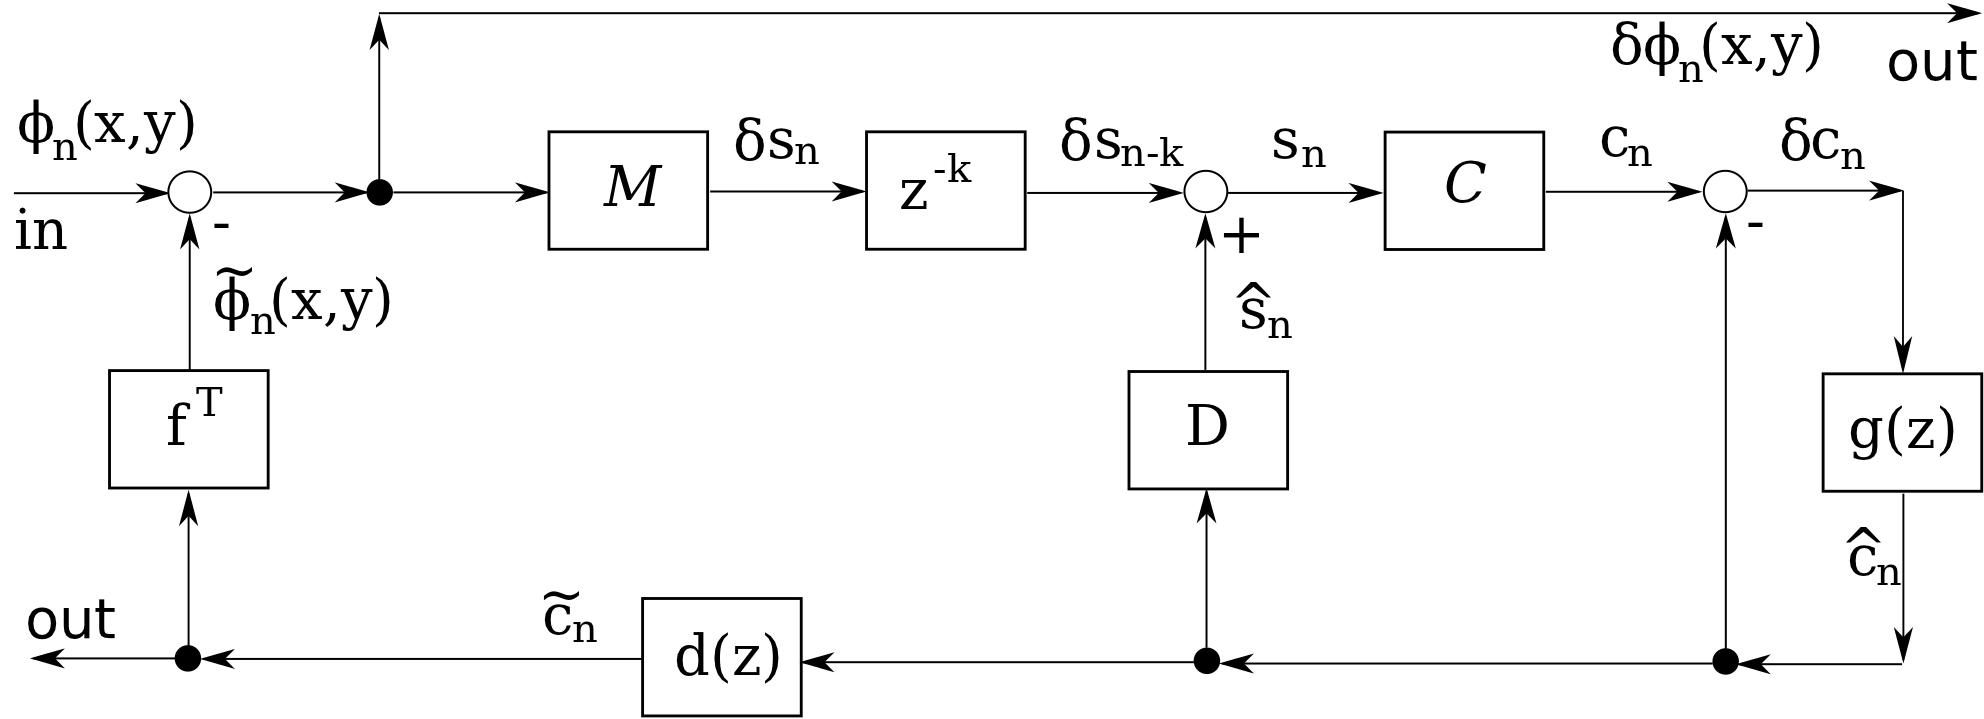
\includegraphics[width = 0.8\textwidth]{POL.png}
\end{center}
\caption{Pseudo Open-Loop MMSE controller block diagram.}
\label{fig:POL}
\end{figure}

The set of dynamic equations for the POL controller is:
\begin{align}
  \texttt{(pseudo open-loop measurement)} \nonumber \\
	\bm{s}(n) = \delta \bm{s}(n-k) + \hat{\bm{s}}(n); \label{eq:POL-meas} \\
	\texttt{(pseudo open-loop command)} \nonumber \\
  \bm{c}(n) = \mathcal{C} \bm{s}(n); \label{eq:POL-est} \\
  \texttt{(command increment)} \nonumber \\
  \delta \bm{c} = \bm{c}(n) - \hat{\bm{c}}(n); \\
  \texttt{(integrator/corrector state space equations, see Appendix
  \ref{app:DF})} \nonumber \\
  \bm{x}^{g}(i+1) = \mathcal{A}^{g} \bm{x}^{g}(n) +
                    \mathcal{B}^{g} \delta \bm{c}(n), \\
  \hat{\bm{c}}(n) = \mathcal{C}^{g} \bm{x}^{g}(n) +
                    \mathcal{D}^{g} \delta \bm{c}(n); \\
  \texttt{(pseudo open-loop measurement estimate)} \nonumber \\
  \hat{\bm{s}}(n) = \mathcal{D} \hat{\bm{c}}(n).
\end{align}
Two important transfer functions (matrices) can be derived from the Fig.
\ref{fig:POL} diagram: 1) the transfer from WFS output $\delta \bm{s}(n)$ to
controller output $\hat{\bm{c}}(n)$ (\emph{controller transfer function}):
\index{controller transfer function}
\begin{equation} \label{eq:WFS-to-Control}
	(\delta \bm{s} \rightarrow \hat{\bm{c}})_{POL}(z) =
	z^{-2} g(z) \left[ \mathcal{I} +
	g(z) (\mathcal{I}-\mathcal{RD}) \right]^{-1} \mathcal{C},
\end{equation}
and 2) the error rejection transfer function:
\begin{equation} \label{eq:phase-to-error}
	(\phi \rightarrow \delta \phi)_{POL}(z) =
	\left[ \mathcal{I} + d(z) \bm{f}^{T}
	(\delta \bm{s} \rightarrow \hat{\bm{c}})_{POL}(z) \mathcal{D} \right]^{-1}.
\end{equation}

Being formally equivalent, feedforward, feedback and POL controllers have
different stability and error propagation properties.

\subsection{Tomographic MMSE reconstructor}
\label{subsec:MMSE-tomo}

\mbox{}

A generalization of the single-conjugate AO control is the \emph{star-oriented
tomography}. \index{star-oriented tomography} The AO control problem is
restated as:
\begin{itemize}
  \item Given is a set of thin phase screens (PS)
  $\{ \phi^{t}_{PS}(\bm{x}) \}_{t=1}^{\#PS}$
  located at a number of altitudes above the telescope and representing the
  atmospheric
  turbulence on the path from a light sources to the telescope aperture.

  \item Likewise, given is a set of phase screens $\{ \phi^{m}_{DM}(\bm{x})
  \}_{m=1}^{\#DM}$ representing the corrections by several DMs that are
  conjugated to a number of altitudes above the telescope. Each DM phase
  screen is a linear combination of the DM influence functions:
	\begin{equation} \label{eq:mcao-dm-inf}
		\phi^{m}_{DM}(\bm{x}) = \bm{f}_{m} (\bm{x}) \bm{c}_{m},
	\end{equation}
	where $\bm{f}_{m} (\bm{x})$ are the $m^{th}$ DM influence function set,
	$\bm{c}_{m}$ is the $m^{th}$ DM control command vector.

  \item There are $\#TAR$ scientific targets to be imaged. Associated with
  each target and each PS or DM is a set
  $( \{ \mathcal{T}^{PS}_{lt} \}_{l=1,t=1}^{\#TAR,\#PS},
     \{ \mathcal{T}^{DM}_{lm} \}_{l=1,m=1}^{\#TAR,\#DM} )$
  of the \emph{propagation operators}
  \index{propagation operator} that map PS or DM phase distributions to the
  wavefront phase distribution in the telescope entrance pupil. With
  assumption that these operators are linear, which is justified for weak
  turbulence, the phase from $l^{th}$ light source in the entrance pupil due to
  all PS phase distortions and all DM phase corrections is
  \begin{equation} \label{eq:mcao-pupil-phase}
    \delta \phi^{l}_{0}(\bm{x}) =
    \sum_{t=1}^{\#PS}
    \mathcal{T}^{PS}_{lt}(\phi_{PS}^{t}(\bm{x})) -
    \sum_{m=1}^{\#DM}
    \mathcal{T}^{DM}_{lm}(\phi_{DM}^{m}(\bm{x})),
    \,\, l = 1,...,\#TAR.
	\end{equation}

	\item Likewise, there are $\#REF$ reference sources feeding light to
	wavefront sensors conjugated to the telescope entrance pupil. Associated
	with the reference sources as well as the PSs and DMs are the propagation
	operators
	$( \{ \mathcal{R}^{PS}_{st} \}_{s=1,t=1}^{\#REF,\#PS},
     \{ \mathcal{R}^{DM}_{sm} \}_{s=1,m=1}^{\#REF,\#DM} )$
	mapping PS or DM phase distributions to the
  wavefront phase distribution in the sensor conjugate exit pupils. The
  closed-loop phase distribution on an $s^{th}$ sensor due to all PS phase
  distortions and all DM phase corrections is
  \begin{equation} \label{eq:mcao-sensor-phase}
    \delta \phi^{s}(\bm{x}) =
    \sum_{t=1}^{\#PS}
    \mathcal{R}^{PS}_{st}(\phi_{PS}^{t}(\bm{x})) -
    \sum_{m=1}^{\#DM}
    \mathcal{R}^{DM}_{sm}(\phi_{DM}^{t}(\bm{x})),
    \,\, s = 1,...,\#REF.
	\end{equation}
	Correspondingly, the $s^{th}$ sensor (closed-loop) readouts are
	\begin{equation} \label{eq:mcao-sensor-read}
		\delta \bm{s}_{s} = \mathcal{M}_{s} (\delta \phi^{s}(\bm{x})),
	\end{equation}
	where $\mathcal{M}_{s}$ is the measurement opertor associated with $s^{th}$
	sensor.

	\item The goal of the tomographic AO control is: given a set of sensor
	measurements $\bm{s} = \{ \bm{s}_{s} \}_{s=1}^{\#REF}$ find the commands
	on all the DMs such that to minimize
	\begin{equation} \label{eq:mcao-cost}
		\langle J \rangle_{\phi,n} =
	  \sum_{l=1}^{\#TAR}
	  w_{l} \langle || \delta \phi_{0}^{l} ||^{2} \,|\, \bm{s} \rangle_{\phi,n},
	  \,\, \sum_{l=1}^{\#TAR} w_{l} = 1,
	\end{equation}
	where $\bm{w} = \{ w_{l} \}_{l=1}^{\#TAR}$ is the set of \emph{target
	direction relative
	weights} \index{target direction weights} and the conditional expectation
	(estimator) is taken over the joint
	statistics of the turbulence layers and the sensor noise.

\end{itemize}

For compactness of notation we introduce the following concatenations:
\begin{itemize}
	\item Propagation operator matrices
	\begin{equation} \label{eq:ps-tar-matrix}
		\mathcal{T}^{PS} = \{ \mathcal{T}^{PS}_{lt} \}_{l=1,t=1}^{\#TAR,\#PS};
	\end{equation}
	\begin{equation} \label{eq:dm-tar-matrix}
		\mathcal{T}^{DM} = \{ \mathcal{T}^{DM}_{lm} \}_{l=1,m=1}^{\#TAR,\#DM};
	\end{equation}
	\begin{equation} \label{eq:ps-ref-matrix}
		\mathcal{R}^{PS} = \{ \mathcal{R}^{PS}_{st} \}_{s=1,t=1}^{\#REF,\#PS};
	\end{equation}
	\begin{equation} \label{eq:dm-ref-matrix}
		\mathcal{R}^{DM} = \{ \mathcal{R}^{DM}_{sm} \}_{s=1,m=1}^{\#REF,\#DM}.
	\end{equation}

	\item Phase vectors
	\begin{equation} \label{eq:ps-vector}
    \bm{\phi}_{PS} (\bm{x}) = \{ \phi_{PS}^{t} (\bm{x}) \}_{t=1}^{\#PS};
	\end{equation}
	\begin{equation} \label{eq:dm-vector}
    \bm{\phi}_{DM} (\bm{x}) = \{ \phi_{DM}^{m} (\bm{x}) \}_{m=1}^{\#DM};
	\end{equation}
	\begin{equation} \label{eq:ps-dm-tar-vector}
    \delta \bm{\phi}_{0} (\bm{x}) =
    \{ \delta \phi_{0}^{l} (\bm{x}) \}_{l=1}^{\#TAR};
	\end{equation}
	\begin{equation} \label{eq:ps-dm-ref-vector}
    \delta \bm{\phi} (\bm{x}) =
    \{ \delta \phi^{s} (\bm{x}) \}_{s=1}^{\#REF}.
	\end{equation}

	\item Sensor measurement vector
	\begin{equation} \label{eq:mcao-meas}
		\delta \bm{s} =
		\{  \mathcal{M}_{s} (\delta \phi^{s}(\bm{x})) \}_{s=1}^{\#REF}.
	\end{equation}

	\item DM influence matrix and control command vector
	\begin{equation} \label{eq:mcao-inf}
		\mathcal{F} (\bm{x}) = \texttt{diag} \{ \bm{f}_{m} (\bm{x}) \}_{m=1}^{\#DM};
	\end{equation}
	\begin{equation} \label{eq:mcao-command}
		\bm{c} = \{ \bm{c}_{m} \}_{m=1}^{\#DM}.
	\end{equation}

	\item Target direction weighting matrix
  \begin{equation} \label{eq:direction-weight}
		\mathcal{W} = \texttt{diag} \{ w_{l} \}_{l=1}^{\#TAR},
	\end{equation}
	and the \emph{weighted norm} \index{weighted norm}
	\begin{equation} \label{eq:weighted-norm}
		|| \bm{\phi} ||^{2}_{\mathcal{W}} =
		\sum_{i} w_{i} || \bm{\phi}_{i} ||^{2} =
		[ \bm{\phi}^{T}, \mathcal{W} \bm{\phi} ].
	\end{equation}

\end{itemize}
In this notation the minimization problem for the cost function given in Eq.
(\ref{eq:mcao-cost}) can be written as
\begin{equation} \label{eq:mcao-minimization}
	\hat{\bm{c}} = \arg \min_{\forall \bm{c}}
	\langle
	||
	\mathcal{T}^{PS} (\bm{\phi}_{PS}) -
	\mathcal{T}^{DM} (\mathcal{F}^{T}) \bm{c}
	||^{2}_{\mathcal{W}} \,|\, \bm{s}
	\rangle_{\phi,n},
\end{equation}
which is a tomographic analog of Eq. (\ref{eq:joint-minimization}).

The tomographic analog to the deterministic DM fitting problem is then stated
as: find the control commands $\hat{\bm{c}}$ for all DMs such that
\begin{equation} \label{eq:tomo-dm-fitting}
	\hat{\bm{c}} = \arg \min_{\forall \bm{c}}
	||
	\mathcal{T}^{PS} (\bm{\phi}_{PS}) -
	\mathcal{T}^{DM} (\mathcal{F}^{T}) \bm{c}
	||^{2}_{\mathcal{W}}.
\end{equation}
To derive solution to this problem we first consider the matrix analog to the
orthogonality principle Eq. (\ref{eq:deterministic-orthogonality-principle}).
Replace each influence function $f_{i}(\bm{x})$ with e.g. a finite vector of
its values on the entrance pupil point grid:
$$ f_{i}(\bm{x}) \rightarrow \bm{f}_{i} = \{ f_{i}(\bm{x}_{j}) \}_{j=1,\#PT},
   \,\, i = 1,...,\#ACT. $$
Then $ \bm{f}^{T}(\bm{x}) \bm{c} \rightarrow \mathcal{F}^{T} \bm{c} $, where
$\mathcal{F}^{T} = [\bm{f}_{1} \,...\, \bm{f}_{\#ACT}]$ and the matrix form
of Eq. (\ref{eq:deterministic-orthogonality-principle}) reads as
\begin{equation} \label{eq:matrix-orthogonality-principle}
	\mathcal{F} (\bm{x}_{0} - \mathcal{F}^{T} \bm{c}) = 0,
	\,\, \bm{x}_{0} = \{ \phi_{0}(\bm{x}_{j}) \}_{j}^{\#PT}.
\end{equation}
Applying this to Eq. (\ref{eq:tomo-dm-fitting}) one derives by analogy
\begin{equation} \label{eq:tomo-dm-fit}
  [ ( \mathcal{T}^{DM} (\mathcal{F}^{T}) )^{T},
	    \mathcal{T}^{PS} (\bm{\phi}_{PS}) -
		  \mathcal{T}^{DM} (\mathcal{F}^{T}) \bm{c} ) ]_{\mathcal{W}} = 0
\end{equation}
and
\begin{equation} \label{eq:tomo-dm-fit}
  \hat{\bm{c}} =
  [ (\mathcal{T}^{DM} (\mathcal{F}^{T}))^{T},
		 \mathcal{T}^{DM} (\mathcal{F}^{T}) ]^{-1}_{\mathcal{W}}
  [ (\mathcal{T}^{DM} (\mathcal{F}^{T}))^{T},
		 \mathcal{T}^{PS} (\bm{\phi}_{PS}) ]_{\mathcal{W}},
\end{equation}
where the \emph{weighted Hilbert metric} is defined as
\index{weighted Hilbert metric}
\begin{equation} \label{eq:weighted-Hilbert-metric}
	[\bm{a}(\bm{x}),\bm{b}(\bm{x})]_{\mathcal{W}} =
	[ \bm{a}^{T}(\bm{x}), \mathcal{W} \bm{b}(\bm{x}) ],
\end{equation}
$[*,*]$ is the usual Hilbert space metric. Correspondingly, the controllable
part of the phase in the entrance pupil for all the target directions is
\begin{equation} \label{eq:tomo-controllable}
	\hat{\bm{\phi}}_{0} = \mathcal{T}^{DM} (\mathcal{F}^{T}) \hat{\bm{c}}.
\end{equation}

The tomographic phase estimation problem is stated as: find the estimate of
phase $\tilde{\bm{\phi}}_{0}$ in entrance pupil for all the target
directions such that
\begin{equation} \label{eq:tomo-phase-estimation}
	\tilde{\bm{\phi}}_{0} = \arg \min_{\forall \mathcal{E}}
	\langle
	||
	\mathcal{T}^{PS} (\bm{\phi}_{PS}) -\mathcal{E} \bm{s}
	||^{2}_{\mathcal{W}}
	\rangle_{\phi,n}
\end{equation}
with the solution written by analogy with Eq. (\ref{eq:phase-estimate})
\begin{equation} \label{eq:tomo-phase-estimate}
  \tilde{\bm{\phi}}_{0} =
  \langle
  \mathcal{T}^{PS} (\bm{\phi}_{PS}) \bm{s}^{T}
  \rangle_{\phi,n}
  \langle
  \bm{s} \bm{s}^{T}
  \rangle_{\phi,n}^{-1} \bm{s}.
\end{equation}
Finally, according to the separation principle, the tomographic
reconstructor generates the estimate $\hat{\tilde{\bm{\phi}}}_{0}$ optimal in
the sense of Eq. (\ref{eq:mcao-minimization}) by substitution of Eq.
(\ref{eq:tomo-phase-estimate}) into Eq. (\ref{eq:tomo-dm-fit}) and then into
Eq. (\ref{eq:tomo-controllable}). This completes the description of a general
tomographic star-oriented AO system.

The GMT LTAO system can be described as a group of inter-connected tomographic
AO subsystems. The detailed mapping of the AO control theory developed in the
previous sections onto the GMT LTAO is given in the next section.

\subsection{GMT LTAO sub-systems}
\label{subsec:ltao-sub-systems}

\mbox{}

According to the \emph{split control concept} \index{split control concept}
the entire GMT LTAO system can be viewed as a set of weakly interacting
control sub-systems (feedback loops, see Fig. 4-35 in Ref.
\cite{GMT-LTAO-CODR}):
\begin{enumerate}
	\item The \emph{ASM high order LGS-based} (ASM HO LGS) \index{ASM high order
	LGS-based control loop}
	control loop intended to reject high spatial order atmospheric/telescope
	aberrations and using the LGS return for WFS measurements. This channel has
	the following features:
	\begin{itemize}
		\item This channel works in closed-loop behind ASM.
		\item Target is $\phi_{Sc}$ is the wavefront from a scientific object.
		\item Reference is $\phi_{LGS}$ is the wavefront from 6 LGSs.
	  \item The control commands generated in this channel are sent to the ASM.
	  \item The wavefront sensors for this channel are the 6 LGS WFSs.
	  \item The sampling rate is the one of the LGS WFSs.
	\end{itemize}

	\item The \emph{ASM low order NGS-based} (ASM LO NGS) or ``truth'' control
	loop is used to provide low order ASM correction, which is impossible to
	determine from the LGSs. Another possible use of the LO NGS WFS is to sense
	the primary segment differential pistons. \index{ASM low order NGS-based
	control loop} This channel has the following features:
	\begin{itemize}
		\item This channel works in closed-loop behind ASM and OI DM.
		\item Target is the wavefront $\phi_{Sc}$ from a scientific object.
		\item Reference is the wavefront $\phi_{NGS}$ from one NGS.
	  \item The control commands generated by this channel are sent to ASM.
	  \item The wavefront sensor for this channel is the LO NGS WFS (``truth
	  sensor'').
		\item The sampling rate is the one of the LO NGS WFS.
	\end{itemize}

	\item The \emph{ASM tip/tilt NGS-based} (ASM TT NGS) \index{ASM tip/tilt
	NGS-based control loop} control loop
	intended to sense and correct the waveront tip/tilt in the scientific object
	direction using a natural guide star. This channel has
	the following features:
	\begin{itemize}
		\item This channel works in closed-loop behind ASM and OI DM.
		\item Target is the wavefront $\phi_{Sc}$ from a scientific object.
		\item Reference is the wavefront $\phi_{NGS}$ from one NGS.
		\item The control commands generated in this channel are sent to the ASM.
		\item The wavefront sensor for this channel is a quad-cell tip/tilt NGS
		(TT NGS) WFS.
	  \item The sampling rate is the one of the TT WFS.
	\end{itemize}

  \item The \emph{OI DM high order LGS-based} (OI DM HO LGS)
  \index{OI DM high order LGS-based control loop} control loop is for
  correcting the NGS wavefront by the OI DM in order to improve performance of
  the NGS TT channel. This channel has the following features:
  \begin{itemize}
	  \item This channel works in closed-loop behind ASM.
	  \item Target is the wavefront $\phi_{NGS}$ from a NGS.
	  \item Reference is the wavefront $\phi_{LGS}$ from 6 LGSs.
	  \item The control commands generated in this channel are sent to OI DM.
	  \item The wavefront sensors for this channel are the 6 LGS WFSs.
    \item The control algorithm is closed-loop with respect to the ASM but
    open-loop with respect to OI DM.
	  \item The sampling rate is the one of the LGS WFSs.
	\end{itemize}

	\item The \emph{OI DM low order NGS-based} (OI DM LO NGS) control loop is
	to provide the low order OI DM correction, which is not possible to
	determine from the LGSs.  \index{OI DM low order NGS-based control loop}
	This channel has the following features:
	\begin{itemize}
		\item This channel works in closed-loop behind ASM and OI DM.
		\item Target is the wavefront $\phi_{NGS}$ from a NGS.
		\item Reference is the wavefront $\phi_{NGS}$ from the same NGS.
		\item The control commands generated by this channel are sent to OI DM.
	  \item The wavefront sensor for this channel is the LO NGS WFS.
		\item The sampling rate is the one of the LO NGS WFS.
	\end{itemize}

\end{enumerate}

One has also to mention some auxiliary control channels used for or together
with LTAO. They are not based on the standard AO control and use other control
approaches.
\begin{enumerate}
	\item \emph{LGS focus stabilization subsystem} \index{LGS focus stabilization
	subsystem} is used for adjusting the LGS WFS
	module focal plane to follow slow LGS position changes in the sky. This
	channel has the following features:
	\begin{itemize}
		\item The feedback signal is the global focus mode extracted from the 6
		LGS WFS measurements.
		\item The control is applied to a servo actuator moving the whole LGS WFS
		module to adjust to the focus. The controller needs to be optimized to the
		(actuator + LGS module) dynamics.
	\end{itemize}
	\item \emph{LGS pupil de-rotation subsystem} \index{LGS pupil de-rotation
	subsystem} is used for compensation of the exit
	pupil rotation on the LGS module induced by changes in the telescope pointing.
	This channel has the following features:
	\begin{itemize}
		\item The feedback signal for this channel is the correlated part of the
		LGS WFS spot motions.
		\item The control is applied to a servo actuator rotating the whole LGS
		WFS module to adjust to the pupil rotation.
	\end{itemize}
	\item \emph{OI WFS acquisition/image stabilization subsystem} \index{OI WFS
	acquisition/image stabilization subsystem} is used find the NGS
	in the telescope field-of-view, to point the light from an NGS to the
	OI WFS detectors and stabilize it. This channel has the following features:
	\begin{itemize}
		\item An acquisition camera is used to provide a signal to the controller.
		\item The control is applied to a two degree-of-freedom actuator attached
		to the acquisition flat mirror located inside OI WFS module.
		\item The acquisition camera and mirror work in closed-loop regime behind
		ASM and OI DM.
	\end{itemize}
	\item \emph{GMT phasing subsystem} \index{GMT phasing subsystem} is an
	\emph{active optics} system that keeps the telescope aligned, phased and
	shape-stabilized.
\end{enumerate}
The auxiliary control sub-systems do not directly participate in the AO
correction but the errors in these systems become the additional error inputs
for the main AO controllers thus upsetting indirectly the AO system
performance.

%!!!!!!
%Let the low order wavefront part to be removed from the wavefront $\bm{x}_{Sc}$
%by the $\mathcal{P}_{HO}$-matrix or extracted from $\bm{x}_{Sc}$ by the
%$\mathcal{P}_{LO}$-matrix can be presented as a linear combination
%$$
  %\bm{x}_{LO} = \sum_{i=1}^{L} w_{i} \bm{q}_{i}
%$$
%of the mutually orthonormal modes $\{ \bm{q}_{i} \}_{i=1}^{L}$, then the
%projection matrices are:
%\begin{eqnarray} \label{eq:l0-ho-projectors}
	%\mathcal{P}_{LO} &=& \mathcal{QQ}^{T}, \\
	%\mathcal{P}_{HO} &=& \mathcal{I} - \mathcal{QQ}^{T}, \\
	%\mathcal{Q} &=& [\bm{q}_{1} \, ... \, \bm{q}_{L}], \,\,
	%\mathcal{Q}^{T} \mathcal{Q} = \mathcal{I}.
%\end{eqnarray}
%In case $\{ \bm{q}_{i} \}_{i=1}^{L}$ are not orthonormal but linearly
%independent, they can be easily orthonormalized by means of the
%QR-decomposition.
%!!!!!! \\

\subsection{GMT LTAO models}
\label{subsec:LTAO-models}

\mbox{}

This section describes elements of the GMT LTAO system mathematical
description: signals, commands, matrices, operators, transfer functions.

\subsubsection{LTAO system element models}
\label{subsubsec:ltao-elements}

GMT LTAO system is a version of the star-oriented tomographic controller with
several channels as described in the previous section. The main physical parts
of the system that need to be modeled together with their interaction are:
\begin{enumerate}
  \item Six (6) Laser Launch Telescopes (LLT) generating six off-axis,
  finite-altitude \texttt{Na}
  Laser Guide Stars (LGS) in regular pattern in the sky. The LGS geometry is
  described in detail in Sec. \ref{sec:lgs}. Table \ref{tab:lgs-parameters}
  gives approximate (subject to change in the course of development)
  parameters of the GMT LGS reference light sources.
	\begin{table}[htp]
	\begin{center}
	\begin{tabular}{c|cccccc}
	\hline

	\hline
    & 1 & 2 & 3 & 4 & 5 & 6 \\
	\hline

	\hline
  $x_{l}^{t}$, m &&&&&& \\
  $y_{l}^{t}$, m &&&&&& \\
  $z_{l}^{t}$, m &&&&&& \\
  \hline
  $\alpha_{l}^{t}$, rad &&&&&& \\
  $\beta_{l}^{t}$, rad &&&&&& \\
  \hline
  $h_{\texttt{Na}}$, m & \multicolumn{6}{|c}{$90 \times10^{3}$} \\
	\hline

	\hline
	\end{tabular}
	\end{center}
	\caption{GMT LGS parameters: $(x,y,z)_{l}^{t}$ -- $l^{th}$ LLT location
	coordinates with respect to GMT entrance pupil; $(\alpha,\beta)_{l}^{t}$ --
	$l^{th}$ LLT direction (first and second Euler angles)
	with respect to GMT
	optical axis; $h_{\texttt{Na}}$ -- mean altitude of the \texttt{Na} layer.
	See Sec. \ref{sec:lgs} for details about the notation.}
	\label{tab:lgs-parameters}
	\end{table}

	\item One (1) infinite-altitude Natural Guide Star (NGS) for tip/tilt and
	possibly other low order aberration sensing. It can be located anywhere
	within 2$^{\prime\prime}$ telescope field of view. Note that the NGS is a
	reference source for the LGS channel and also both target and reference
	source for the On-Instrument WFS channel.

	\item One infinite-altitude (1) Science Target (ST) light source to be
	imaged through LTAO
	system. Normally it is assumed to be on the GMT optical axis but we reserve
	a possibility for it to be at $(\alpha,\beta)^{t}_{ST} \neq 0$ off-axis
	direction (first and second Euler angles) with respect to the optical axis.

	\item Atmospheric turbulence propagation path. It is parameterized by the
	$C_{n}^{2}$ profile, wind profile, split in to a number of discrete
	turbulence phase screens (PS) located at altitudes
	$\{ h_{s} \}_{s=1}^{\#PS}$, with the covariance functions
	$\{ \langle \phi^{PS}_{s}(\bm{x}_{1},\bm{x}_{2}) \rangle \}_{s=1}^{\#PS}$,
	where $\bm{\phi}^{PS} (\bm{x}) = \{ \phi^{PS}_{s}(\bm{x}) \}_{s=1}^{\#PS}$
	are the instantaneous phase distributions on the
	screens (see details in Section \ref{sec:atmosphere}).
	Propagation from the target and reference light sources through the
	atmosphere is described through the propagation operator matrices:
	\begin{itemize}
		\item $\mathcal{T}_{ST}^{PS}$ -- propagates light from the scientific
		target through turbulence phase screen phase distributions
		$\bm{\phi}^{PS}(\bm{x})$ to the entrance pupil.
		\item $\mathcal{R}_{LGS}^{PS}$ -- propagates light from the 6 LGSs
		through turbulence phase screen phase distributions
		$\bm{\phi}^{PS}(\bm{x})$ to the entrance pupil.
		\item $\mathcal{R}_{NGS}^{PS}$ -- propagates light from the NGS
		through turbulence phase screen phase distributions
		$\bm{\phi}^{PS}(\bm{x})$ to the entrance pupil.
	\end{itemize}

	\item GMT entrance pupil. It is parameterized through:
	\begin{itemize}
		\item Pupil location $(x,y,z)^{g}_{t}$ and orientation
		$(\alpha,\beta)_{t}^{g}$ coordinates with respect to the
		laboratory coordinate system (see Sec. \ref{sec:lgs}). The
		\item Pupil shape (see Ref. \cite{ConanGMTmath}).
	\end{itemize}

	\item GMT deformable mirrors:
	\begin{itemize}
		\item Adaptive Secondary Mirror (ASM). It is parameterized by the set of
		influence functions $\bm{f}_{ASM}$ and DM phase screen
		$\phi_{DM}(\bm{x})$ conjugated to altitude $h_{ASM} = TBD$ and the
		ASM transfer matrix
		$\mathcal{H}_{ASM}(z)$ responsible for the mirror dynamics.
		\item Analogously, the On-Instrument Deformable Mirror (OI DM) is
		parameterized through $\bm{f}_{DM}$,
		$\phi_{DM}(\bm{x})$, $h_{DM} = TBD$, $\mathcal{H}_{DM}(z)$.
	\end{itemize}
	Light propagation from the target and reference sources through ASM and
	DM phase screens to the entrance pupil is described by propagation operator
	matrices:
	\begin{itemize}
		\item $\mathcal{T}_{ST}^{DM}$ -- propagates light from the scientific
		target through OI DM to the entrance pupil.
		\item $\mathcal{T}_{ST}^{ASM}$ -- propagates light from the scientific
		target through ASM to the entrance pupil.
		\item $\mathcal{R}_{LGS}^{ASM}$ -- propagates light from the 6 LGSs
		through ASM to the entrance pupil.
		\item $\mathcal{R}_{NGS}^{DM}$ -- propagates light from the NGS
		through OI DM to the entrance pupil.
		\item $\mathcal{R}_{NGS}^{ASM}$ -- propagates light from the NGS
		through ASM to the entrance pupil.
	\end{itemize}
  More details on the GMT deformable mirrors can be found in Sec. \ref{sec:dm}.

	\item There are three (3) wavefront sensors:
	\begin{itemize}
		\item LGS HO WFS consisting of 6 sensor blocks. It is described by poke
		matrix $\mathcal{D}_{LGS}^{ASM}$ for interaction between LGS HO WFS
		and ASM, sensor noise covariance matrix
		$\langle \bm{n}_{LGS}^{} \bm{n}_{LGS}^{T} \rangle$, anti-aliasing filter
		operator $\mathcal{P}_{LGS}$ for action of the LGS HO WFS field
		stops on the input wavefront phase.
		\item NGS TT WFS described by matrix $\mathcal{D}_{TT}^{ASM}$ describing
		interaction between NGS TT WFS
		and ASM, poke matrix $\mathcal{D}_{TT}^{DM}$ for interaction between NGS
		TT WFS and the OI DM, sensor noise covariance matrix
		$\langle \bm{n}_{TT}^{} \bm{n}_{TT}^{T} \rangle$, anti-aliasing filter
		operator $\mathcal{P}_{TT}$ describing action of the NGS TT WFS field
		stop on the input wavefront phase.
		\item NGS LO WFS described by matrix $\mathcal{D}_{LO}^{ASM}$ for
		interaction between NGS TT WFS
		and ASM, poke matrix $\mathcal{D}_{LO}^{DM}$ for interaction between NGS
		LO WFS and the OI DM, sensor noise covariance matrix
		$\langle \bm{n}_{LO}^{} \bm{n}_{LO}^{T} \rangle$, anti-aliasing filter
		operator $\mathcal{P}_{LO}$ describing action of the NGS LO WFS field
		stop on the input wavefront phase.
	\end{itemize}
	More details on the GMT wavefront sensors can be found in
	Sec. \ref{sec:sh-wfs}.

	\item The following signals circulate in the system:
	\begin{itemize}
		\item $\bm{\phi}_{PS}^{}(\bm{x})$ -- instantaneous phase distortions on the
		atmospheric turbulence phase screens.
		\item $\bm{\phi}_{ASM}^{}(\bm{x})$ -- instantaneous phase corrections on the
		ASM.
		\item $\bm{\phi}_{DM}^{}(\bm{x})$ -- instantaneous phase corrections on the
		OI DM.
		\item $\delta \bm{\phi}^{HO}_{ST} (\bm{x}) = \mathcal{T}^{PS}_{ST}
		(\bm{\phi}_{PS}^{}) - \mathcal{T}^{ASM}_{ST} (\bm{\phi}_{ASM}^{})$
		-- instantaneous phase distribution in the entrance pupil from
		atmospheric turbulence and ASM corrections propagated from the Science
		Target. This is the scientific target wavefront seen in the LGS HO WFS
		channel and, up to
		non-common path aberrations, in the scientific instrument channel.
		\item $\delta \bm{\phi}^{OI}_{ST} (\bm{x}) = \mathcal{T}^{PS}_{ST}
		(\bm{\phi}_{PS}^{}) - \mathcal{T}^{ASM}_{ST} (\bm{\phi}_{ASM}^{}) -
		\mathcal{T}^{DM}_{ST} (\bm{\phi}_{DM}^{})$
		-- instantaneous phase distribution in the entrance pupil from
		atmospheric turbulence and both ASM and OI DM corrections propagated from
		the Science Target. This is the scientific target wavefront seen in the OI
		WFS channel.
		\item $\delta \bm{\phi}_{LGS}^{HO} (\bm{x}) = \mathcal{R}^{PS}_{LGS}
		(\bm{\phi}_{PS}^{}) - \mathcal{R}^{ASM}_{LGS} (\bm{\phi}_{ASM}^{})$
		-- instantaneous phase distribution in the entrance pupil from both
		atmospheric turbulence and DM corrections propagated from the 6 LGSs. This
		is the reference source wavefront(s) seen in the LGS HO WFS channel.
		\item $\delta \bm{\phi}^{HO}_{NGS} (\bm{x}) = \mathcal{R}^{PS}_{NGS}
		(\bm{\phi}_{PS}^{}) - \mathcal{R}^{ASM}_{NGS} (\bm{\phi}_{ASM}^{})$
		-- instantaneous phase distribution in the entrance pupil from
		atmospheric turbulence and ASM corrections propagated from the Science
		Target. This is the NGS wavefront seen in the LGS HO WFS
		channel and used as a target for the OI DM control algorithm.
		\item $\delta \bm{\phi}_{NGS}^{OI} (\bm{x}) = \mathcal{R}^{PS}_{NGS}
		(\bm{\phi}_{PS}^{}) - \mathcal{R}^{ASM}_{NGS} (\bm{\phi}_{ASM}^{}) -
		\mathcal{R}^{DM}_{NGS} (\bm{\phi}_{DM}^{})$
		-- instantaneous phase distribution in the entrance pupil from
		atmospheric turbulence and both ASM and DM corrections propagated from the
		NGS. This is the reference source wavefront seen in the OI WFS channel.
		\item $\delta \bm{s}_{LGS}^{} = \mathcal{M}^{LGS} \mathcal{P}_{LGS}
		(\delta \bm{\phi}_{LGS}^{HO}) + \bm{n}_{LGS}^{}$
		-- instantaneous LGS HO WFS readout, where $\mathcal{M}_{LGS}$ is exact
		(infinite-dimensional) LGS HO WFS measurement operator, $\bm{n}_{LGS}^{}$ is
		the instantaneous LGS HO WFS noise readout.
		\item $\delta \bm{s}_{TT}^{} = \mathcal{M}^{TT} \mathcal{P}_{TT}
		(\delta \bm{\phi}_{NGS}^{OI}) + \bm{n}_{TT}^{}$
		-- instantaneous NGS TT WFS readout, where $\mathcal{M}_{TT}$ is exact
		(infinite-dimensional) NGS TT WFS measurement operator, $\bm{n}_{TT}^{}$ is
		the instantaneous NGS TT WFS noise readout.
		\item $\delta \bm{s}_{LO}^{} = \mathcal{M}^{LO} \mathcal{P}_{LO}
		(\delta \bm{\phi}_{NGS}^{OI}) + \bm{n}_{LO}^{}$
		-- instantaneous NGS LO WFS readout, where $\mathcal{M}_{LO}$ is exact
		(infinite-dimensional) NGS LO WFS measurement operator, $\bm{n}_{LO}^{}$ is
		the instantaneous NGS LO WFS noise readout.
		\item $\bm{c}_{ASM}^{} = \bm{c}^{TT}_{ASM} + \bm{c}^{LO}_{ASM} +
		\bm{c}^{HO}_{ASM}$ -- instantaneous ASM control command vector consisting
		of tip/tilt (TT), low order (LO) and high order (HO) corrections.
		\item $\bm{c}_{DM}^{} = \bm{c}^{LO}_{DM} + \bm{c}^{HO}_{DM}$ --
		instantaneous OI DM
		control command vector consisting of low and high order corrections.
		\item $\bm{c}_{LGS}^{}$ -- instantaneous LGS control command vector
		consisting of LGS WFS platform focus and rotation commands and the 6 LLT
		tip/tilt corrections.
	\end{itemize}
	\item The following projection operators are used for channel splitting:
	\begin{itemize}
		\item $\mathcal{P}_{ST}^{HO}$ -- spatial high-pass projection operator
		acting on the $\delta \bm{\phi}_{ST}^{HO}$ wavefront.
		\item $\mathcal{P}_{ST}^{LO}$ -- spatial low-pass projection operator
		acting on the $\delta \bm{\phi}_{ST}^{HO}$ wavefront.
		\item $\mathcal{P}_{NGS}^{HO}$ -- spatial high-pass projection operator
		acting on the $\delta \bm{\phi}_{NGS}^{HO}$ wavefront.
		\item $\mathcal{P}_{NGS}^{LO}$ -- spatial low-pass projection operator
		acting on the $\delta \bm{\phi}_{NGS}^{OI}$ wavefront.
		\item $\mathcal{P}_{NGS}^{TT}$ -- spatial low-pass projection operator
		extracting tip/tilt from the $\delta \bm{\phi}_{NGS}^{OI}$ wavefront.
	\end{itemize}

\end{enumerate}
The vectors, matrices and operators listed above are the
building blocks for the LTAO system control algorithms ans simulations. Below
we elaborate on the internal structure of these objects.

\subsubsection{Phase screens and propagation operators}
\label{subsubsec:phase-and-propagation}

As it was described in Sec. \ref{subsec:MMSE-tomo}, the phase
distribution vector $\vec{\phi}(\bm{x})$, is a concatenation of the
turbulence distributions $\phi(\bm{x})$ on each phase screen,
where $\bm{x}$ are the $(x,y)^{t}$-coordinates in the $t$-system (see Sec.
\ref{sec:lgs}) in the case of the phase screens being perpendicular to
the telescope optical axis regardless of the pointing, which we will assume
throughout this document. The phase distribution vector
$\bm{\phi} (\bm{x})$ in the entrance pupil, where $\bm{x}$ are the
pupil $(x,y)^{t}$-coordinates, is a concatenation of phase distributions
corresponding to propagation from the several target or reference sources.
Because of the assumed linearity of the propagation operators, propagation
operator matrices $\mathcal{T}$ or $\mathcal{R}$ are
block $\#SRC\times\#PS$ matrix, where $\#SRC$ is the number of sources and
$\#PS$ is the number of phase screens. Each block $ij$ of the propagation matrix
is a scalar propagation operator mapping phase distribution on the $j^{th}$
phase screen to the entrance pupil propagated from $i^{th}$ source. Thus, the
operators involved in the GMT LTAO model are
\begin{itemize}
	\item $\mathcal{T}_{ST}^{PS}$ is a $1 \times \#PS$-matrix;
	\item $\mathcal{R}_{LGS}^{PS}$ is a $6 \times \#PS$-matrix;
	\item $\mathcal{R}_{NGS}^{PS}$ is a $1 \times \#PS$-matrix;
	\item $\mathcal{T}_{ST}^{ASM}$ and $\mathcal{T}_{ST}^{DM}$ are $1 \times
	1$-matrices and, to simplify equation for $\delta \bm{\phi}_{ST}^{OI}$, these
	two matrices can be concatenated into one $1 \times 2$-matrix
	$\mathcal{T}_{ST}^{OI}$;
	\item $\mathcal{R}_{NGS}^{ASM}$ and $\mathcal{R}_{NGS}^{DM}$ are $1 \times
	1$-matrices and, to simplify equation for $\delta \bm{\phi}_{NGS}^{OI}$, these
	two matrices can be concatenated into one $1 \times 2$-matrix
	$\mathcal{R}_{NGS}^{OI}$.
\end{itemize}

The $\mathcal{T}$ and $\mathcal{R}$ propagation operators have especially
simple form in case of the geometrical optics propagation (see Section
\ref{sec:lgs}):
\begin{equation} \label{eq:shift-propagator}
	\mathcal{H}(\bm{\phi}(\bm{x})) = \bm{\phi}(a\bm{x}+\bm{b}),
\end{equation}
where $\mathcal{H}$ stands either for $\mathcal{T}$ or $\mathcal{R}$ and
$(a,\bm{b})$ are computed from Eq. (\ref{eq:pupil-to-layer}) for finite
altitude point source (LGS) or Eq. (\ref{eq:pupil-to-layer-inf}) for infinite
altitude point source (TS or NGS).

\subsubsection{Projection operators}
\label{subsubsec:projection-operators}

For the ideal channel split the following relations hold:
\begin{equation} \label{eq:HO-split}
	\mathcal{I} = \mathcal{P}_{ST}^{HO} + \mathcal{P}_{ST}^{LO},
\end{equation}
\begin{equation} \label{eq:HO-LO-TT-split}
	\mathcal{I} = \mathcal{P}_{NGS}^{HO} + \mathcal{P}_{NGS}^{LO} +
	              \mathcal{P}_{NGS}^{TT}.
\end{equation}
Thus, only three projection operators out of five need to be computed. Since
all the splitting projection operators act on the wavefront phase from a single
light source (ST or NGS) $\mathcal{P}$ are $1 \times 1$-matrices or just
scalar operators.

Let an
orthonormal basis $\bm{q}(\bm{x}) = \{ q_{i}(\bm{x}) \}_{i=1}^{\infty} $ be
defined on the entrance pupil domain $A$ with the basis functions
$q_{i}(\bm{x})$.
Then an orthogonal projector on a subset $ \{ q_{i}(\bm{x}) \}_{i \in S} $ is
\begin{equation} \label{eq:orthogonal-projector-def}
	\mathcal{P}^{S} ( \phi(\bm{x}) ) = \bm{q}^{T}_{S} [\bm{q}_{S}^{},\phi],
\end{equation}
where $\bm{q}_{S}^{} (\bm{x}) = \{ q_{i} (\bm{x}) \}_{i \in S}$, $[*,*]$ is the
Hilbert space metric defined in Eq. (\ref{eq:Hilbert-metric}). If the basis
functions are sorted in ascending order with respect to the abundance of high
order details, then the $\mathcal{P}^{TT}$-operators are made of
$\{ q_{1},q_{2} \}$ (and, hopefully, $q_{1}(\bm{x})$ and $q_{2}(\bm{x})$ are
indeed are very similar to tip and tilt, which is not guaranteed for a
segmented aperture), the $\mathcal{P}^{TT}$-operators are made of
$\{ q_{3}, ..., q_{LO}^{} \}$, etc.

%In the following sections details of the subsystem control algorithms are
%discussed. We concentrate there on the non-dynamic algorithm versions to
%highlight the basic operation flow and the data structures involved. The
%algorithm modifications to account for the dynamic effects are postponed to
%the later sections. Note, however, that the information about the non-dynamic
%algorithms is higly reusable in the dynamic versions.

\subsection{ASM HO LGS controller algorithm}
\subsection{ASM LO NGS controller algorithm}
\subsection{ASM TT NGS controller algorithm}
\subsection{OI DM HO LGS controller algorithm}
\subsection{OI DM LO NGS controller algorithm}

\subsection{GMT LTAO system fusion}
\label{subsec:ltao-system-fusion}

TBD

\subsection{GMT LTAO system dynamic analysis}
\label{subsec:ltao-dynamics}

TBD

\subsection{GMT LTAO system error and robustness analysis}
\label{subsec:ltao-errors}

TBD